
% TODO
\section{Client}
\subsection{Überblick}
\begin{frame}[<+-| alert@+>]{QNut}
	\begin{itemize}
		\item nahezu vollständige Steuerung des Servers über die Library
		\item Steuerung des wpa\_supplicant ebenfalls über die Library
		\item benutzerspezifische Skripte möglich
		\item Feedback für den Benutzer
	\end{itemize}
\end{frame}


\subsection{QNut}
\begin{frame}[<+-| alert@+>]{Hauptfenster}

		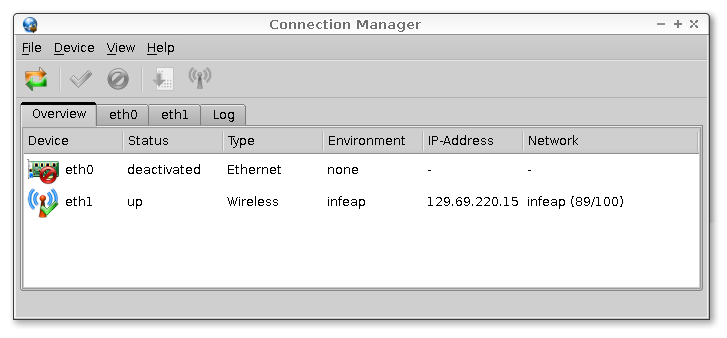
\includegraphics[scale=0.25]{qnut_overview.png}
		% qnut_overview.png: 727x338 pixel, 72dpi, 25.65x11.92 cm, bb=0 0 727 338

	\begin{itemize}
		\item Übersichten für Devices, Environments und Drahtlosnetzen
		\item Aktueller Status
	\end{itemize}
\end{frame}

\begin{frame}[<+-| alert@+>]{Steuerung und Skripte}

		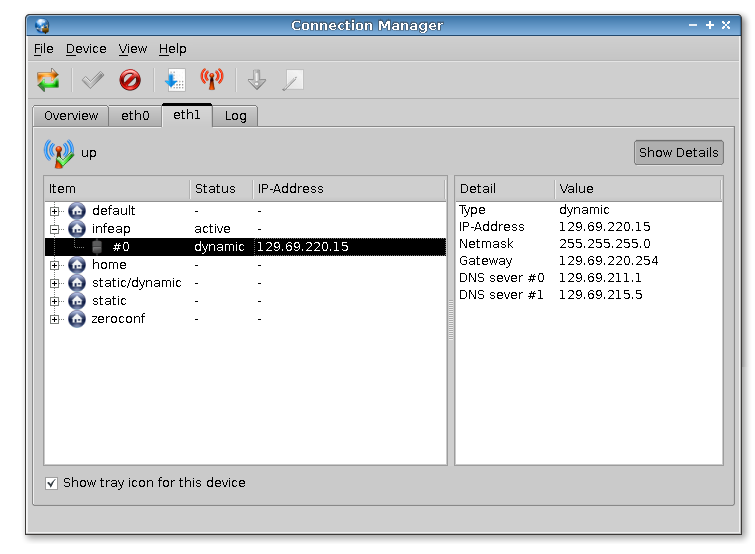
\includegraphics[scale=0.25]{qnut_detailed.png}
		% qnut_detailed.png: 755x554 pixel, 72dpi, 26.63x19.54 cm, bb=0 0 755 554

	\begin{itemize}
		\item Detailansichten für Environments und Interfaces
		\item Auswahl eines aktiven Environments
		\item Konfiguration eines Interaces
	\end{itemize}
\end{frame}

\begin{frame}[<+-| alert@+>]{Steuerung und Skripte}

		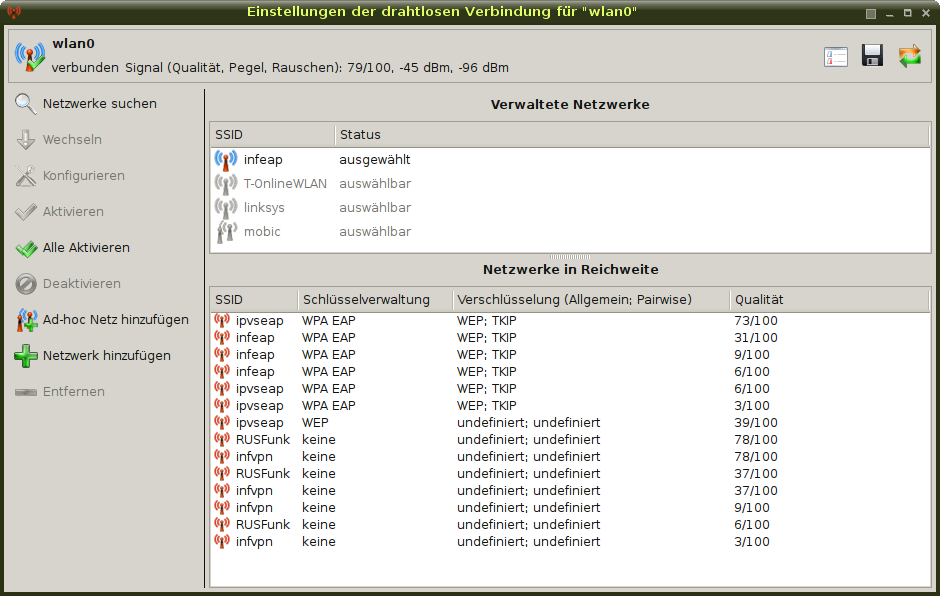
\includegraphics[scale=0.25]{qnut_scan.png}
		% qnut_scan.png: 952x651 pixel, 72dpi, 33.58x22.97 cm, bb=0 0 952 651

	\begin{itemize}
		\item Anpassung der verwalteten Drahtlosnetze
		\item Scannen nach vorhandenen Drahtlosnetzen
	\end{itemize}
\end{frame}

\begin{frame}[<+-| alert@+>]{Steuerung und Skripte}

		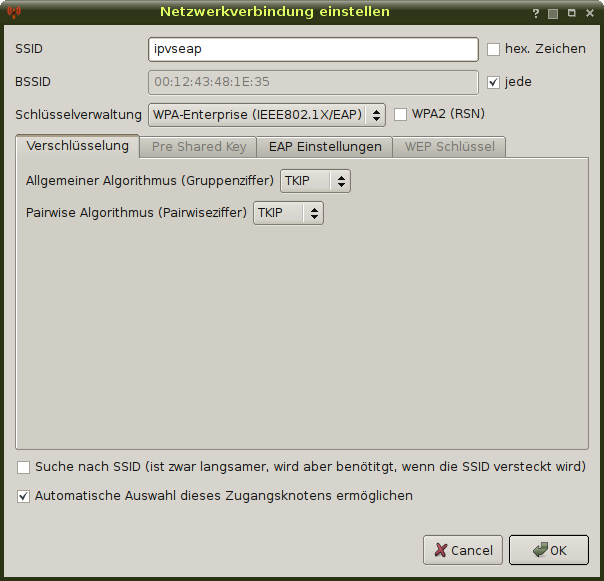
\includegraphics[scale=0.25]{qnut_netconfig.png}
		% qnut_netconfig.png: 523x602 pixel, 72dpi, 18.45x21.24 cm, bb=0 0 523 602

	\begin{itemize}
		\item Hinzufügen und Entfernen von Drahtlosnetzen
		\item Konfiguration vorhandener Netzwerke
	\end{itemize}
\end{frame}


\begin{frame}[<+-| alert@+>]{Sonstiges}

	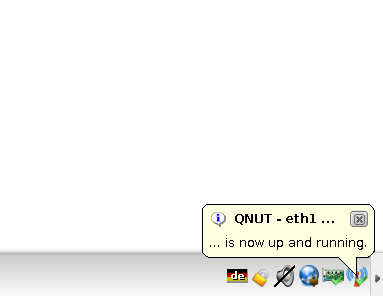
\includegraphics[scale=0.25]{qnut_tooltip.png}
	% qnut_tooltip.png: 383x296 pixel, 72dpi, 13.51x10.44 cm, bb=0 0 383 296

	\begin{itemize}
		\item Tray-Icon zum schnelleren Zugang
		\item Statusänderung der Devices als Tool-Tip
		\item Ausführung von Skripten je Devicestatus
	\end{itemize}
\end{frame}



